\documentclass[12pt]{beamer}
\usetheme{LMT}
\usepackage[utf8]{inputenc}
\usepackage{amsmath}
\usepackage[makeroom]{cancel}
\usepackage{xcolor}

\setbeamertemplate{footline}[frame number]{}

\newcommand\Ccancel[2][black]{\renewcommand\CancelColor{\color{#1}}\bcancel{#2}}

\pdfinfo
{
  /Title       (Presentation Reunion)
  /Author      (Pierre NARGIL)
}

\newcommand\FontReduce{\fontsize{8}{10}\selectfont}
\newcommand\FontReduceT{\fontsize{9}{11}\selectfont}


\title{Avancement du travail}
\subtitle{Présentation hebdomadaire}
\author{Pierre Nargil}

\graphicspath{{figures/}}
% ---------------------------------------------------------------------
\begin{document}


\frame{\titlepage}

\frame{\tableofcontents}


\section{Rappels de la dernière réunion}

	\begin{frame}
	
		\frametitle{Rappels de la dernière réunion}
		%\framesubtitle{Un sous titre}
		
		\begin{itemize}
			\item Les questions abordées :
			\begin{itemize}
				\only<1>{\FontReduce}
				\item Expliquer la différence sur le cas analytique
						\\ 	\only<2>{\textcolor{blue}{Évolution du programme de François depuis la présentation.}}
				\item \textcolor<-1>{red}{Pour réutiliser les modes trouvés par SVD, comment trouver les fonctions en temps associées ?}
						\\ 	\only<3>{\textcolor{blue}{...}}
				\item \textcolor<-1>{red}{Le 1er mode de la 1ère itération est-il  la répose statique dde l'effort moyen ?}
			\end{itemize}
			
			\only<-1>{
				\item Les objectifs de travail à court terme :
				\begin{itemize}
					\FontReduce
					\item \textcolor<-1>{red}{Mettre en place une résolution Newton-Raphson pour l'élément non-linéaire.}
					\item \textcolor<-1>{red}{Effectuer un SVD sur la solution obtenue par PGD, comparer avec les résultat précédents.
																	Et une Orthogonalisation}
					\item Comparaison du cas analytique haute fréquence
					\item \textcolor<-1>{red}{Évaluer le rôle de l'amortissement du schéma par rapport à l'amortissement du problème 
																	dans la stagnation de l'erreur PGD}
					\item \textcolor<-1>{red}{Lecture HOSVD}
					\item \textcolor<-1>{red}{Test SVD sur matrice 2x2 symbolique pondérée}
					
				\end{itemize}
			}
		\end{itemize}

	\end{frame}

%\section{Point de travail - avancement}

%\section{Questions soulevées}
\section{Constats et Remarques}
	
	
\section{Modifications dans le programme}
%	\begin{frame}
%		\frametitle{Modifications dans le programme}
%		\begin{itemize}
%			\item $\bullet$ A
%			\item $\circ$ U
%				\begin{itemize}
%					\FontReduce
%					\item Le 
%				\end{itemize}
%		\end{itemize}
%	\end{frame}

%\subsection{Presudo-programme}
%\subsection{Cas test}
%\subsection{Equations}
\section{Objectifs de travail}

	\begin{frame}
	
		\frametitle{Objectifs de travail}
			\framesubtitle{Comparaison du cas analytique haute fréquence}
				\begin{figure}
					\only<1>{
						Résultat de François
						\\
						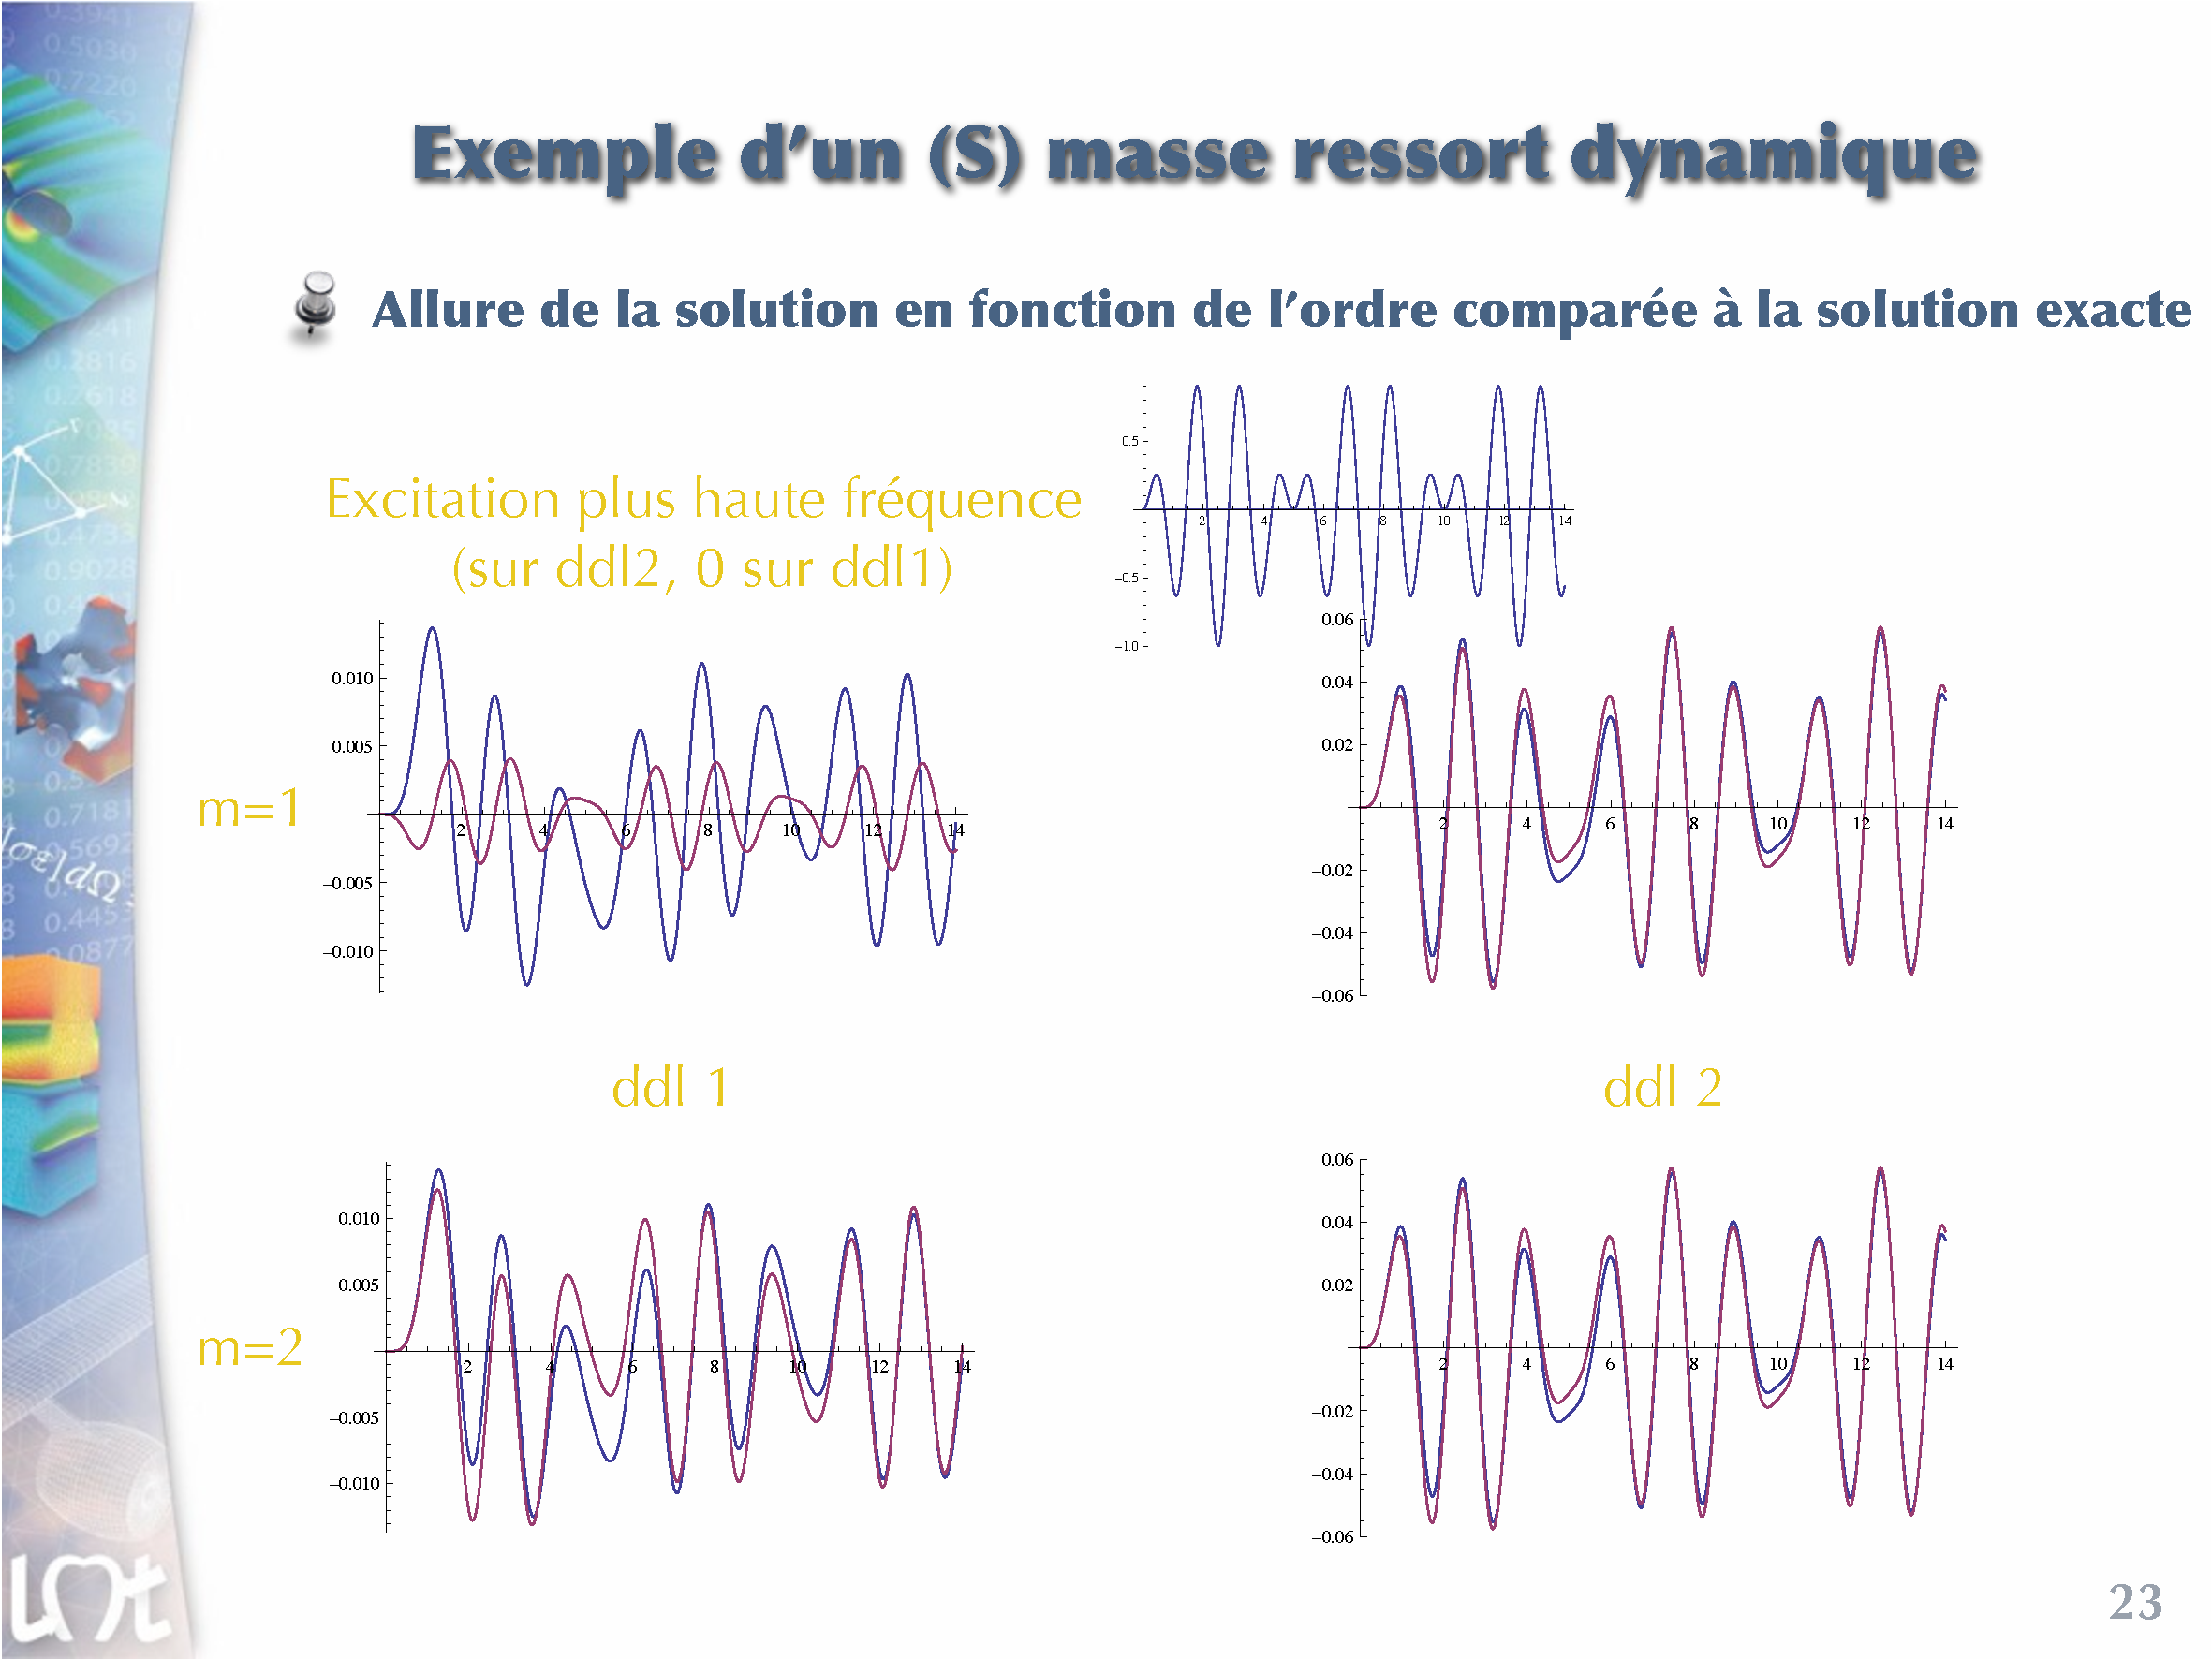
\includegraphics[trim=3cm 2cm 3cm 11cm, clip=true,width=\linewidth ,keepaspectratio]{Reduction_Modele_Francois.pdf}				
					}
					\only<2>{
						Résultat de mon programme
						\\
						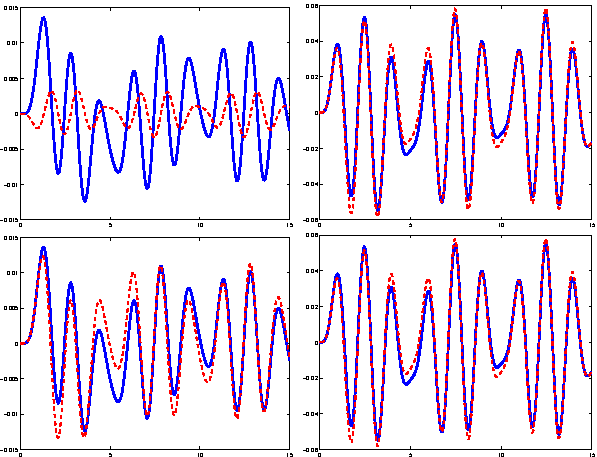
\includegraphics[width=\linewidth, height=6cm ,keepaspectratio]{Analytic.pdf}
					}
					\only<3>{
						\begin{itemize}
							\item Correspondance parfaite :
									\begin{itemize}
										\item La solution converge vers la solution exacte
										\item Les deux premiers modes trouvés sont identiques
									\end{itemize}
							\item 8 modes $\Rightarrow$ erreur $< 1\%$
							\item Point Fixe :
							\begin{itemize}
								\item convergence apres 4 iterations
								\item convergence apres 3 iterations
							\end{itemize}
						\end{itemize}
						
					}
				\end{figure}
	\end{frame}
	
	\begin{frame}
		\frametitle{Objectifs de travail}
		\framesubtitle{3 méthodes - Analyse de Mac}
		\only<1>{
			\begin{figure}
				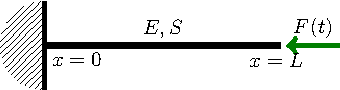
\includegraphics[width=0.5\linewidth ,keepaspectratio]{Beam-tikz-0.pdf}				
				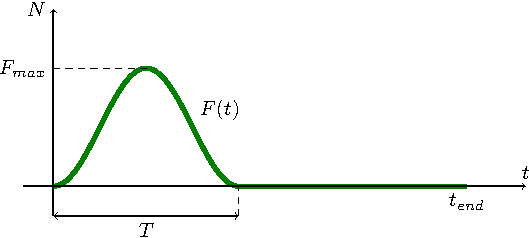
\includegraphics[width=0.5\linewidth ,keepaspectratio]{SinVerse-tikz.pdf}	
			\end{figure}
		}
		\only<2>{
			\centering  SVD(PGD) - POD
			\\
			\vspace{0.5cm}
			\hspace{-1.2cm}
			\raisebox{-0.5\height}{	
				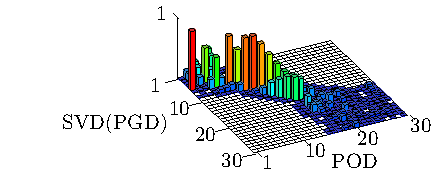
\includegraphics[trim=1cm 0cm 0cm 0cm, clip=true,width=0.55\linewidth ,keepaspectratio]{MacSVD(PGD)-POD.pdf}
				}
			\hspace{-0.7cm}
			\raisebox{-0.5\height}{	
				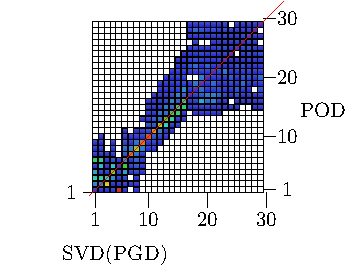
\includegraphics[trim=0.5cm 0cm 0cm 0cm, clip=true,width=0.55\linewidth ,keepaspectratio]{MacSVD(PGD)-POD-2.pdf}
				}
			\hspace{-1.5cm}
		}
		\only<3>{
			\centering  SVD(Solution PGD) - POD
			\\
			\vspace{0.5cm}
			\hspace{-1.2cm}
			\raisebox{-0.5\height}{	
				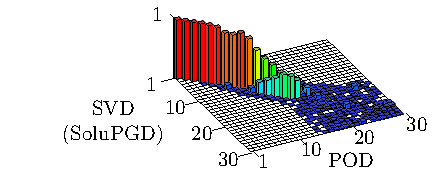
\includegraphics[trim=1cm 0cm 0cm 0cm, clip=true,width=0.55\linewidth ,keepaspectratio]{MacSVD(SoluPGD)-POD.pdf}
				}
			\hspace{-0.7cm}
			\raisebox{-0.5\height}{	
				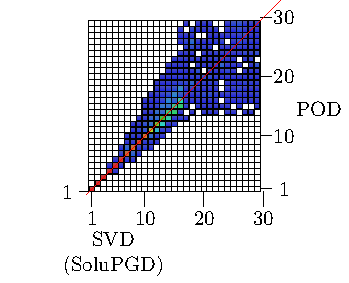
\includegraphics[trim=0.5cm 0cm 0cm 0cm, clip=true,width=0.55\linewidth ,keepaspectratio]{MacSVD(SoluPGD)-POD-2.pdf}
				}
			\hspace{-1.5cm}
		}
		\only<4>{
			\centering  SVD(PGD Ponderee) - POD
			\\
			\vspace{0.5cm}
			\hspace{-1.2cm}
			\raisebox{-0.5\height}{	
				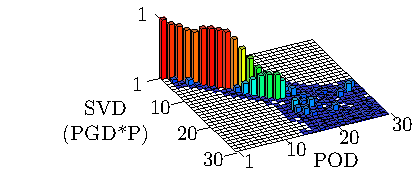
\includegraphics[trim=1cm 0cm 0cm 0cm, clip=true,width=0.55\linewidth ,keepaspectratio]{MacSVD(PGD-Ponderee)-POD.pdf}
				}
			\hspace{-0.7cm}
			\raisebox{-0.5\height}{	
				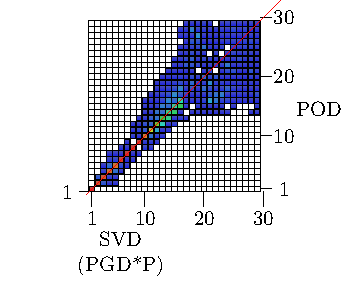
\includegraphics[trim=0.5cm 0cm 0cm 0cm, clip=true,width=0.55\linewidth ,keepaspectratio]{MacSVD(PGD-Ponderee)-POD-2.pdf}
				}
			\hspace{-1.5cm}
		}
	
	\end{frame}
	
\section{Points blocants}

	\begin{frame}
	
		\frametitle{Points blocants}
		\begin{itemize}
			\item PGD - TDG
			\item Orthogonalisation
			\item PGD \& Non-linéaire
				\begin{itemize} 
					\item Comment prendre en compte l'évolution de $ \mathbf{K} $ dans le problème en espace.
				\end{itemize}
			\item Absence d'éléments de comparaison pour les résultats non-linéaire.
		\end{itemize}
	
	\end{frame}

\section{Questions}

%	\begin{frame}
%	
%		\frametitle{Questions}
%		
%		\begin{itemize}
%			\item Pseudo-programme. Une norme ou un logiciel conseillé?
%			\item Comment utiliser des modes trouvés en dehors de la PGD? Faire tourner le point fixe sans modifier le mode espace ?
%		\end{itemize}
%	
%	\end{frame}
	
\section{Programme de travail}

	\begin{frame}
	
		\frametitle{Programme de travail}
		
		\begin{itemize}
			\item Journée Farman
			\item Petit-déj
			\item ...
			\item Differente fréquences F(t) (comparer aux f propre de la poutre) $\Rightarrow$ quand ça diverge
					(Somme de sinus à la place de SinusVerse ?)
			\item SVD(Solution PGD) - Mettre la SVD dans la boucle CalcMode
		\end{itemize}
	
	\end{frame}
%
%
%\begin{frame}
%
%	\frametitle{Prerequisites \& Goals}
%	\framesubtitle{Knowledge is a brick wall that you raise line by line forever}
%	
%	\begin{block}{LaTeX}
%		\begin{itemize}
%			\item Obviously some basic LaTeX knowledge is necessary
%			\item Some more features will be provided here
%		\end{itemize}
%	\end{block}
%	
%	\begin{block}{Beamer}
%		\begin{itemize}
%			\item You'll learn them by looking at this presentation source
%		\end{itemize}
%	\end{block}
%	
%	\begin{block}{Goal}
%		\begin{itemize}
%			\item Learn how to make well structured slides
%			\item Using a beautiful theme
%			\item Take over the world
%		\end{itemize}
%	\end{block}
%
%\end{frame}

\end{document}
% ---------------------------------------------------------------------
